
%TODO Zuviele Kommas ;), im Englischen werden so gut wie keine Kommas verwendet!

%TODO !!!! Sehr wichtig wäre die Überarbeitung des AGI Kapitels. Ich habe gar nicht verstanden, um was es in der Psi Theorie geht und deswegen natürlich auch nicht die Implementierung dazu. Das zieht sich dann auch durch in deine Implementierung und die Case study. Hier empfehle ich dir dringend eine ausführlichere Erklärung!

\chapter{Artificial General Intelligence}
\label{chap:2}
To provide the necessary context for this thesis, this chapter will provide a brief introduction to the corresponding foundations on the AI side.

%TODO !! was ist strong AI? Du kannst nicht davon ausgehen, dass der Leser das weiß

First, we will introduce AGI as a subset of artificial intelligence. Based on this, the Psi theory, as a particular instance of strong AI theories, is described in detail. The description includes a brief history of its concrete implementations. Then, MicroPsi~2, the latest framework dedicated to the Psi theory, is described in detail.

    \section{Strong AI}
    
%TODO Den Satz versteh ich nicht    
    
It took many years for AI research to evolve from the early ideas of thinking machines over Deep Blue, the computer that could beat mankind's best chess players to Watson, the AI that beats the champions of Jeopardy, the game show, that is about asking the appropriate question to a given answer. There exist many applications for AI. Self-driving cars and online-shopping recommendation systems to name a few.

%TODO Zitierung der Quelle der Definitionen?

These examples have one thing in common. They are applications of technology that serves an immediate, or at least foreseeable purpose. For AI in scenarios of this kind, the term \emph{applied AI} (or \emph{weak AI}) has been coined. \emph{Strong AI}, in contrast, is about researching the nature of intelligence itself. An actual (hypothetical) implementation of a strong AI would mean, one would have to build a machine, that is capable of acting like a human being---not just for a limited problem set, but in all of them. 

%TODO feelings? really?

Another term, that is being used more recently, is \emph{AGI}, for \emph{Artificial General Intelligence}. It it is in contrast to what are called \emph{narrow AI} applications, which chess computers and other expert systems would be an excellent example for. AGI sets out, to develop software that can solve and act appropriately in a wide variety of problem fields, without specialising on any particular problem whatsoever. A complete AGI system is supposed to control itself autonomously and to have it's own thoughts and feelings. This has been the original focus of the AI field, before many lost their enthusiasm about it, when it turned out being not as imminently as expected. Even though the advances in narrow AI contribute to it, AGI is more than just an assembly of these. There is a huge number of different AGI projects being worked on, with most of them being in early stages.~\cite{goertzel2007artificial}

%TODO Was ist der Unterschied zwischen strong AI und AGI?

%TODO Versteh ich nicht

Cognitive AI, in particular, can be thought of as architectures that implement findings and theories in the fields cognitive science and psychology, as well as the neurosciences, for the sake of proving, if the theories hold against what they promise. Many cognitive architectures share characteristics with or directly implement artificial neural networks.

%TODO Sollte das nicht bei der Definition von weak und strong AI kommen? Warum erst jetzt? Wieso springst du immer zwischen den Bezeichnungen strong AI and AGI hin und her?

Looking upon the field of AI from a philosophical point of view, computers seem to deliver enormous potential for learning about how minds work. At the same time, new questions arise. If we knew how cognition works and if we could build machines that simulate it, would these minds be real? And what would the ethical implications be? According to Russel's and Norvig's standard reference \emph{Artificial Intelligence: A Modern Approach}~\cite{russell2009artificial}, one can distinguish in between two fundamental assumptions. The assumption that computers are able to act \emph{as if} they were intelligent is called the weak AI hypothesis. Thinking that an intelligently acting machine ,in fact, \emph{is} performing cognition, is called strong AI hypothesis.

Putting it differently, weak AI considers computers to be an instrument to research cognitive processes, whereas strong AI considers simulated cognitive processes as actually being cognition.

%TODO Ab hier ist mir nicht ganz klar, warum du das alles schreibst. Ist schön zu lesen, aber ich erkenne den Beitrag zu deiner Arbeit nicht. Außerdem wirst du hier sehr emotional ;)

Trying to figure out, if machines are able to achieve cognition, we often explain by enumerating things that computers can not to. They can not be kind, friendly or have a sense of humour. Neither can they tell right from wrong, fall in love or learn from experience. But what can they do? They are at least partly involved in almost every significant recent discovery in most sciences. They steer cars safer than we ever did. Where \emph{exactly} to draw the dividing line between intelligence and machinery?~\cite{russell2009artificial}

The most famous indicator for whether a machine is intelligent or not, is the Turing test. Decades after its formulation, contests regarding to it are still being held---may the best conversationalist win! Many would argue that even an algorithm that passes the Turing test would still not be intelligent. It would trick people into thinking it was, but it would still not be conscious, aware of itself. Moreover, it would not have emotions.~\cite{russell2009artificial}

But, would not what we believe is possible and what is not, become obsolete, once we would be able to build something that cognition can not be denied from? 

Eventually, this question, might not be as significant as it appears to be. Dijkstra tried to explain that whether something is able to think or not, is first and foremost a matter of language and the interpretation of the word \emph{think}, when he famously said: ``The question of whether machines can think... is about as relevant as the question of whether submarines can swim.''

    \section{Psi Theory}
    
%TODO !! cite! Originalzitat sehr wichtig!

This section gives an overview of the basic ideas of the Psi theory. The descriptions are based on \emph{Principles of Synthetic Intelligence PSI: An Architecture of Motivated Cognition}~\cite{Bach:2009:PSI:1611304} by Joscha Bach.

The theory in its foundations was first described by German psychologist Dietrich Dörner in his books ``Bauplan für eine Seele''~\cite{Doerner1998} and ``Die Mechanik des Seelenwagens''~\cite{dorner2002mechanik} from 1998 and 2002. Dörner's holistic approach goes beyond classic problem solving and develops a unified model for cognition that implements motivation and emotions. He is convinced that artificial intelligence does not have to focus on different aspects of cognition that have to be looked at separately but that a unified theory will ultimately lead to a deeper understanding of cognition itself.
    
Dörner's ``Bauplan für eine Seele''~\cite{Doerner1998} (``blueprint for a mind'') belongs in the interdisciplinary field Cognitive Science, as with his theory he tries to research psychological foundations with the methods of Computer Science. The theory is an attempt to explain the mind as a machine. It has a notable focus on the emotional system and addresses symbolic and sub-symbolic reasoning.  The mind is looked at as a fuzzy and self-extending causal network structure.

The theory tries to model the human mind as an agent, that is controlled by a structure of relationships and dependencies, that strives to maintain homeostatic balance. Every form of representation in the agent's cognition---may it be percepts, plans or abstractions of space and objects---is represented as directed, hierarchic spreading-activation networks. This structure can be visualised as an artificial neural network, which we will call \emph{node net} in the following. Nodes in these networks have gates that may send activation and slots that may receive it. The basic elements a node net consists of are called \emph{quads}. Quads themselves consist of one central neuron and four outer neurons that are called \emph{sub}, \emph{sur}, \emph{ret} and \emph{por}~(see figure~\ref{quad}). The outer neurons can be connected with the central neurons of other quads and thereby form networks. The four different kinds of outer neurons represent different kinds of relations. \emph{sub} stands for a ``has part'' relationship, \emph{sur} is the inverse to sub an represents an ``is part'' relationship, \emph{ret} stands for the ordering relationship of succession and \emph{por} represents predecession.

\begin{figure}[h]
  \centering
    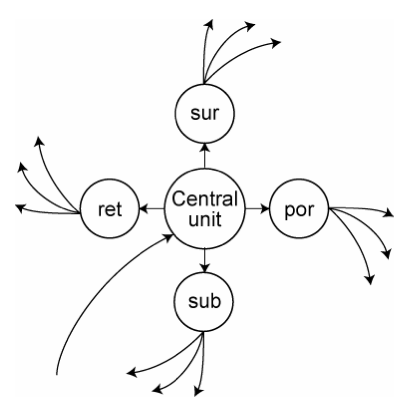
\includegraphics[width=6cm]{graphics/quad}
  \caption{Quads like this are the basic representational unit of the Psi theory (taken from \cite{Bach:2009:PSI:1611304})}
  \label{quad}
\end{figure}

Furthermore each neuron has an activation value, that it receives from and forwards to other neurons. Links in between neurons can be modified to dynamically modulate the forwarded activation value. The modulation of the flow of activation is interpreted as emotions.

There are specific kinds of neurons that are called \emph{sensors} and \emph{actuators}. They represent the in- and output to the outside world. Sensors receive activation if they are triggered by the environment and activated actuators lead to an action in the environment.

The motivation of Psi agents comes from a set of predefined drives. They are divided into physiological (e.g. physical integrity), social (e.g. affiliation) and cognitive drives (e.g. reduction of uncertainty). These drives may signal a specific demand. If the value of a demand changes, pleasure or displeasure signals are sent to the agent. By reinforcement learning agents learn what behaviour leads to the fulfilment of demands. 

As node nets may create new nodes and links on their own, the agent forms memory, motives and plans, that help it to select what action to execute next (see figure~\ref{motive_architecture}). Agents can store representation of their entire percept sequence, but only those that are connected to pleasure or displeasure signals are being kept.

\begin{figure}[h]
  \centering
    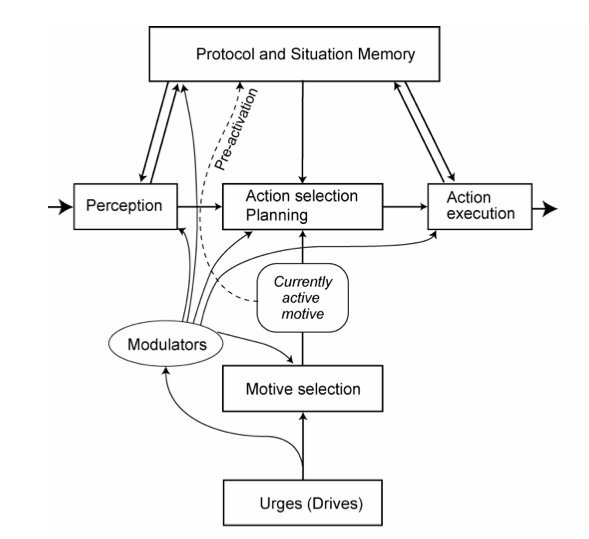
\includegraphics[width=10cm]{graphics/motive_architecture}
  \caption{The basic architecture of action selection in Dörner's theory (taken from \cite{Bach:2009:PSI:1611304})}
  \label{motive_architecture}
\end{figure}

Quads are used to form \emph{partonomies} that represent information about concepts and relationships. A partonomy is a hierarchical structure that represents a part-whole relationship. For example, the concept ``head'' would be represented as the assembly of a face and a head. A face furthermore would itself consist of a mouth, a nose, eyes and so forth~(see figure~\ref{partonomy}). 

Through the combination of partonomies and order relations, all basic types of relationships the agent stores are formed. These could be causal, spatial or temporal relationships in between states of the environment, for example.

\begin{figure}[h]
  \centering
    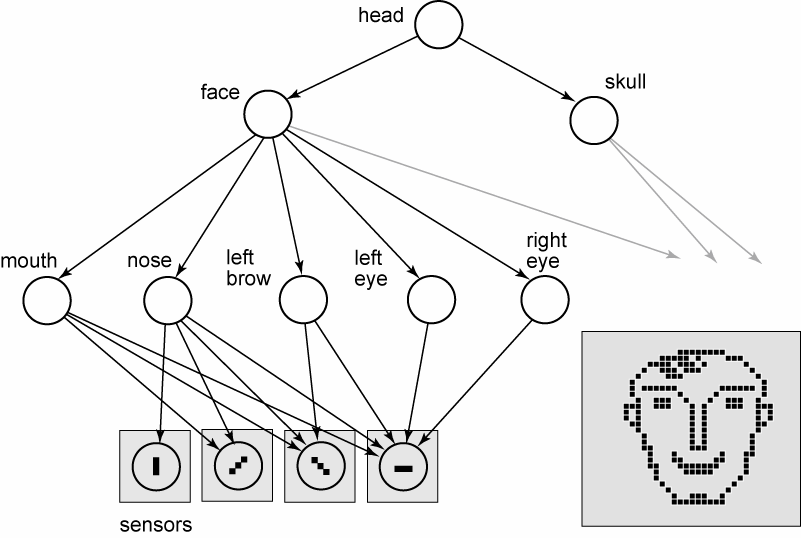
\includegraphics[width=9cm]{graphics/partonomy}
  \caption{The partonomic representation of a Cartoon face (taken from \cite{Bach:2009:PSI:1611304})}
  \label{partonomy}
\end{figure}

Psi agents' basic approach to problem solving works by going through a set of subsequent stages. The agent first tries to approach a problem with behavioural routines. If these do not solve the problem, the agent tries to construct a plan, by trying to find a chain of causal relationships that ultimately lead to a state, that solves the problem. If no plan is found, the agent starts to explore its environment to gather more knowledge.

The goal of implementing the theory to computer software is to find potential inconsistencies and moreover to find out if Psi agents show similar behaviour to that of humans. If they do, the Psi theory could possibly serve as an explanation about how human minds work. For this purpose, a number of experiments---similar to video games---have been concluded, in which both Psi agents and human players had to perform specific tasks. Later on, their behaviours have been compared and searched fir similarities and differences.
 
%TODO !!! Das ist deine Hauptgrundlage!!! Ich habe leider nicht verstanden,was die Grundgedanken sind. Du musst die Grundkonzepte der Theorie vorstellen und in Relation setzen. Was ist die Motivation für die Theorie, was erreicht man damit, wie erreicht man die Ziele? Abbildungen tragen sicherlich auch zum Verständnis bei!

Joscha Bach adapted the theory to bring it in a contemporary form with slight modifications in his dissertation \emph{Principles of Synthetic Intelligence PSI: An Architecture of Motivated Cognition}~\cite{Bach:2009:PSI:1611304}. Even though building a conscious machine that thinks and acts as we do is still mere science-fiction, it is this kind of foundational research, that leads us to new ways of thinking about the world, that give us our most significant leaps.
    
    \section{Agents and Environments}

%also define symbolic and subsymbolic    

Before we continue to describe concrete implementations and simulations, we define agents and environments according to Russel and Norvig.~\cite{russell2009artificial} 

%TODO Ist das ein wörtliches Zitat? Ist besonders zu kennzeichnen!

An \emph{agent} is defined as anything that can perceive its environment through sensors and conduct actions inside the environment through actuators. The examples given in \cite{russell2009artificial} include a software agent that may receive network packets as sensory inputs and produces output by writing files and sending network packets fits in nicely within this thesis. However, agents can just as well be robots that have cameras as sensors and motors as actuators. Even humans can be thought of as agents that perceive their environment through their senses and act upon it through their muscles.

Russel and Norvig furthermore define the \emph{percept}, as the agent's input and the \emph{percept sequence} as the complete history of what the agent has perceived. Each decision an agent makes is based on the percept sequence.

Additionally, they describe the \emph{agent function}, as the function that maps each percept sequence to an action. The \emph{agent program} is its concrete implementation.

A \emph{rational agent} is an agent that acts appropriately to any given percept sequence. To answer the question about what is appropriate and what is not, they introduce \emph{performance measures} that evaluate the agent's actions. These measures have to be defined by the designer of an experiment. Summarising, the rational agent tries to maximise its performance measure at any given point of time.

%TODO Ich frage mich, ob diese Definitionen alle nötig sind. Du solltest später dann darauf eingehen, wie deine konkrete Implementierung im Bezug auf diese Definitionen zu sehen ist.

\emph{Environments} have a number of different properties. They can either be \emph{fully observable} or \emph{partially observable}. An environment is fully observable when the agent has access to the complete state of the environment---or at least to everything that is relevant, regarding to the performance measure. As opposed to this, it is partially observable, if the previously mentioned requirement is not given.

An environment can moreover be \emph{single agent} or \emph{multiagent}. An environment is multiagent, when there is at least one other agent, whose behaviour is about maximising a performance measure that depends on the first agent's behaviour. If the agents try to maximise the performance measure of all agents, the environment is called \emph{cooperative}. If agents try to maximise their own and minimise the performance measure of the other agents, it is called \emph{competitive}.

An environment may furthermore be \emph{discrete} or \emph{continuous}. If an environment can be thought of as advancing from one discrete state to the other, it is discrete (and even more so if there is a finite number of states). If the transitions between states are thought of as being continuous, so is the environment.

A \emph{task environment} is the combination of the performance measure, the environment and the agent's actuators and sensors.

    \section{Psi Implementations}
Psi has been implemented by different groups at different times. The first implementations are by Dörner and his associates themselves~(see figure \ref{psi_screen}). They used Delphi Pascal and developed it for Windows environments. This implementation can still be downloaded (\cite{PsiDownload}) and runs on Windows 7 installations, for example. 

\begin{figure}[h]
  \centering
    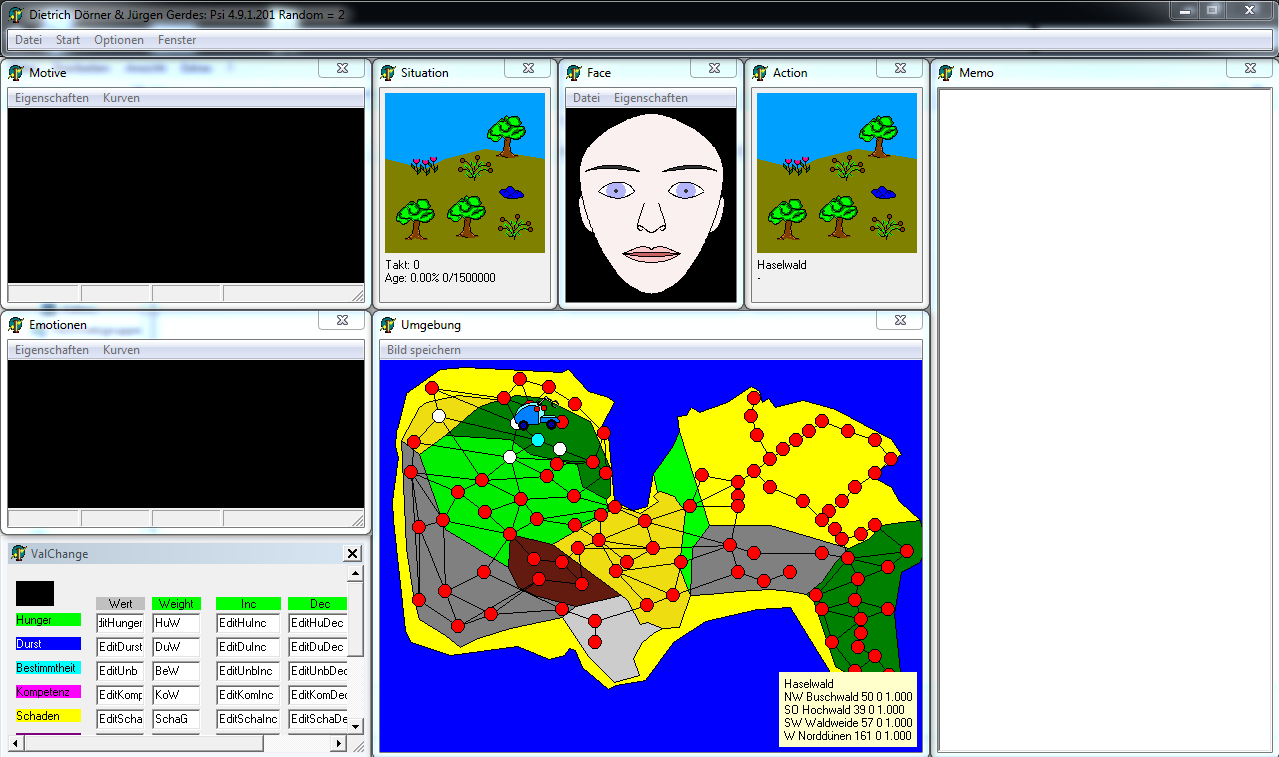
\includegraphics[width=10cm]{graphics/psi_screen1}
  \caption{Screenshot of Dörner's team's Delphi Pascal Psi implementation}
  \label{psi_screen}
\end{figure}

%TODO Was ist das? Vorher nie erwähnt!

Subsequently, there has been a simple 3D implementation of Dörner's island simulation called Psi3D.

%TODO was bedeutet "interfacing the world"?

The work on Dörner's team's implementations has not been continued, so Joscha Bach and his associates developed new implementations of Psi. From 2003 to 2009 they built an implementation in Java as a set of plugins for the Eclipse IDE called MicroPsi. It included a graphical editor and a broad experimentation framework. MicroPsi provided a complex and sophisticated simulation component which contained simulated objects in three dimensional worlds---even though most experiments took place on a plane. As a pragmatic approach, different ground types of the simulation world have been stored in bitmap files similar to height-maps. The framework offered complex administrator interfaces and appealing DirectX rendered 3D-views of the scenery as well as a more general world view which interfaced the world by providing clickable objects. Predefined simulation environments included a classic Island and a Mars world (see figure~\ref{micropsi_3d_screen}). Objects in these worlds may be assembled recursively out of other objects and bring their own functionalities. As it has been the case in Dörner's implementation, a viewer for facial expressions has been included---this time as well as a three-dimensional simulation.~\cite{Bach:2009:PSI:1611304}


\begin{figure}[h]
  \centering
    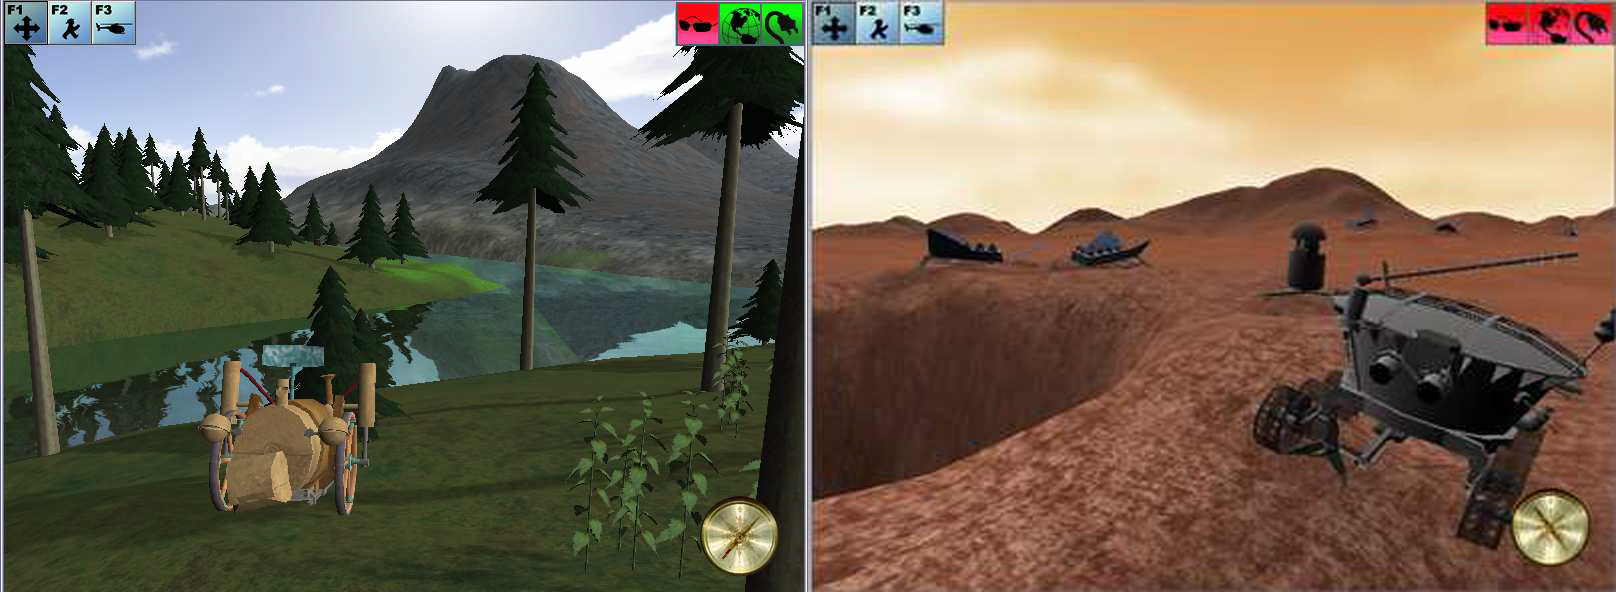
\includegraphics[width=14cm]{graphics/micropsi_3d_screen}
  \caption{Screenshots of the 3D visualisation component in MicroPsi (taken from \cite{Bach:2009:PSI:1611304})}
  \label{micropsi_3d_screen}
\end{figure}

Simulated environments proved especially to serve well for the research of collaborative behaviour of multiple agents, for mapping and exploration, image processing as well as for memory and planning. Additionally, some scenarios, that are almost impossible to implement in the physical world (such as evolving agent populations) could easily be simulated. On the other hand, downsides of simulated worlds include being limited by computing power and the programmer's specifications.~\cite{Bach:2009:PSI:1611304}

    \section{MicroPsi 2}
    \label{sec:2:MicroPsi}
To ensure broad understandability and to maintain platform independence, MicroPsi has been built ground up again in 2011 and 2012 using more lightweight Python code. What is remarkable about the new implementation called MicroPsi 2 (in the following MicroPsi), is that the simulation is deployed as a web application and the graphical interface is completely rendered inside a web browser, using state-of-the-art internet- and web application technologies.~\cite{conf/agi/Bach12}
        
Even though there have been more complex simulation environments (e.g. 3D-worlds) for previous implementations of Psi architectures, the relatively new version of MicroPsi so far has only two fairly simple ones: a 2D-Island and a map of the public transportation system of Berlin~(see figure~\ref{mp2_berlin}). Instead of building a new 3D-world, with this project we set out for something more experimental. More on this follows in chapters three and four.

\begin{figure}[h]
  \centering
    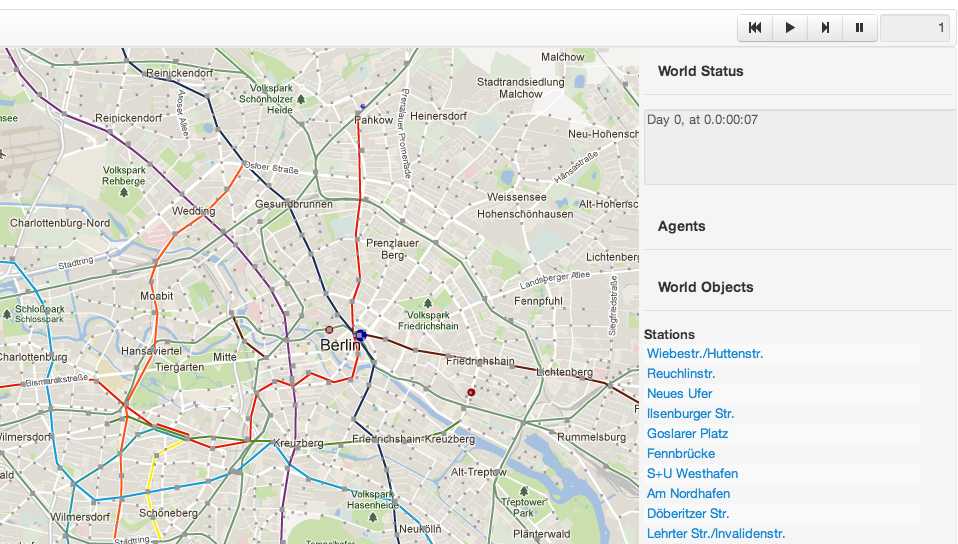
\includegraphics[width=14cm]{graphics/mp2_berlin}
  \caption{MicroPsi's simulation environment Berlin}
  \label{mp2_berlin}
\end{figure}

        \subsection{Module Overview}
        
%TODO world adapter inherit from world object in UML
    
%TODO Was macht so ein node net? Sollte vorher klar werden!

%TODO Wozu? Bitte nur das beschreiben, was du auch erklärst und brauchst (user & config manager)
        
MicroPsi is written in Python with a minimum of dependencies. Therefore, its  modular structure is comparably easy to understand. It is illustrated in figure~\ref{micropsi2_modules}. First, one can differentiate in between the \texttt{Server} module (or the web interface) and the actual simulation \texttt{Runtime} module (also called \emph{core}). In a simple simulation experiment setup, MicroPsi runs three threads: one for the \texttt{Server} and, invoked by the \texttt{Runtime}, one \emph{world runner} that runs a simulation world as well as one \emph{node net runner} that runs a node net. As these names suggest, the \texttt{Runtime} manages both the simulation environments as well as the inhabitant agents (or node net embodiments). They may by design run asynchronously. In fact, the \texttt{Runtime} works entirely independently of the \texttt{Server} and therefore may just as well be deployed for command line interaction or other GUIs. Furthermore, the \texttt{Server} contains a \texttt{UserManager} and the \texttt{Runtime} a \texttt{ConfigurationManager}.~\cite{conf/agi/Bach12}
\\          

%TODO !! Das ist kein UML. An einem Lehrstuhl für Softwaretechnik sollte es das sein. Außerdem sind nicht alle Module erklärt, sowie die Assoziationen erwas unklar
          
\begin{figure}[h]
  \centering
    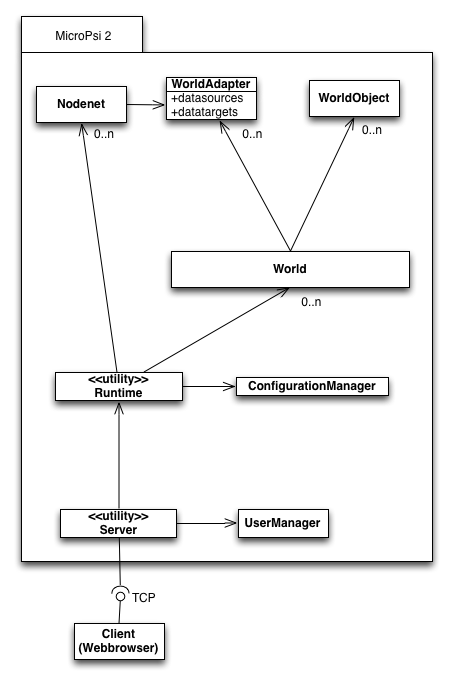
\includegraphics[width=9cm]{graphics/UML_MicroPsi_v12}
  \caption{The modular architecture of the MicroPsi framework makes it easy to extend. (taken from~\cite{conf/agi/Bach12})}
  \label{micropsi2_modules}
\end{figure}

The following description is heavily based on \cite{conf/agi/Bach12}, where the theoretical foundations can be found in detail.

        \subsection{Module \texttt{Server}}
The \texttt{Server} renders the GUI and deploys the agent simulation as a web application. It acts as a web server for remote or local access. A client for this application may be any computer with a reasonable up-to-date web browser. Therefore, simulations can be launched from anywhere without requiring any installation. It rests upon the lightweight Python web framework \emph{Bottle}~\cite{bottlepy}.

The web interface is based on HTML as well as Javascript. The communication in between the browser and the simulation is managed via JSON remote procedure calls. Many GUI components of Twitter's \emph{Bootstrap} library are in use. The graphic renderings (see figure~\ref{micropsi2_nodenet}) utilise the JavaScript graphics library \emph{PaperJS}. 

\begin{figure}[h]
  \centering
    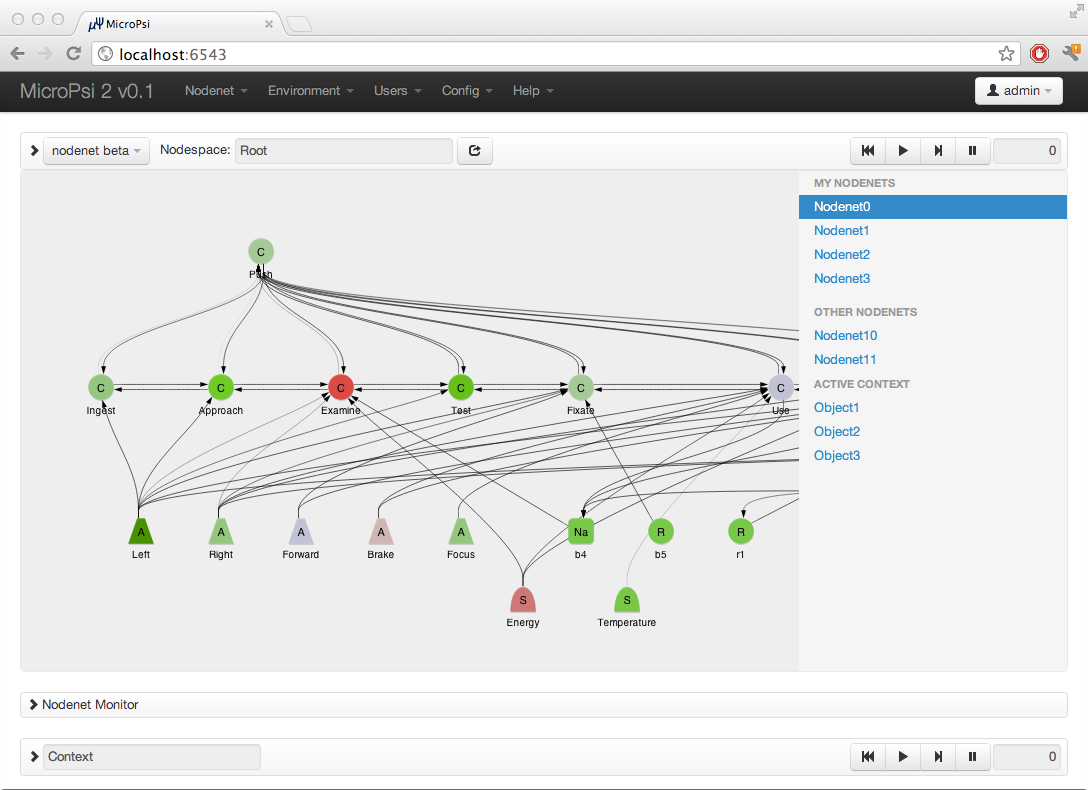
\includegraphics[width=13cm]{graphics/micropsi2_nodenet}
  \caption{The graphical editor is the primary interface to node nets. (taken from~\cite{conf/agi/Bach12})}
  \label{micropsi2_nodenet}
\end{figure}

The \texttt{Server} communicates with its users through the server API. User sessions and access rights are managed by the \texttt{UserManager}.
   
        \subsection{Module \texttt{Runtime}}
In this setup, the \texttt{Server} starts the \texttt{Runtime}---even though it may also work independently of the \texttt{Server}. The \texttt{Runtime} component communicates with the \texttt{Server} through the MicroPsi API. It manages node nets and worlds.

        \subsubsection{Node Nets}

%TODO Wozu knotentypen? wozu benutzt man node nets? Leider verstehe ich das gar nicht
        
A MicroPsi node net is defined as a set of states, a starting state, a network function, that defines how to advance to the next state, and a set of node types. Data sources and data targets serve as the input for nodes and output towards a world, where a data source is filled with data from the world and data targets are linked to agent actions in the world.

According to the Psi theory, nodes may have different types and parameters. They contain gates and slots that send and receive an activation. In most cases, the activation is forwarded from a slot to a gate without further modulation.

Nevertheless, nodes may include functions that enable the creation of new nodes and links as well as procedures for learning and planning. They may be implemented as Python code.

According to the concepts of the Psi theory, MicroPsi defines agents as node nets or to be more specific, hierarchical spreading activation networks. They are an ``abstraction of the information processing provided by brain''~\cite{conf/agi/Bach12}. Agents can be placed and researched in simulation environments or physically embodied as robots.

%TODO cite * 2

%TODO Was willst du damit sagen? Zu kurz!

As node nets share the relevant characteristics with neural networks, they may enable neural learning paradigms. To store information they can form semantic networks. Furthermore, nodes may contain state machines and other operations, which make it possible to build modularised architectures.

        \subsubsection{Worlds}
        \label{microPsiWorld}
The simulations worlds are the environments in which we can study our agent's behaviour. Worlds need to provide a world adapter which functions as the interface in between a node net and the environment. Within the world adapter, data sources and data targets have to be defined carefully, to get a functional and meaningful experiment going. They represent the agent's sensory input and the motoric output. Sophisticated interconnection of those enables interaction with the environment.

The \emph{world adapter} has to define \emph{data sources} and \emph{targets}. It fills the sources with data from the world and writes the targets to the world. The node net does the opposite: it reads from the sources and writes into the targets. This enables a feedback loop in between the world and the node net. Furthermore, the \emph{world adapter} provides a step function, that advances the world and is called by the MicroPsi world runner frequently.


The kind of data the world adapter interfaces, is not specified any further, which gives developers the opportunity to experiment with classic simulation worlds, as well as exotic applications (eg. stock data). At the time of the original development of the MicroPsi, the prioritised application was building a framework for knowledge representation.

            \paragraph{Objects}$\;$ \\
Worlds contain objects. Objects may be anything that could be interesting for a simulation, and that needs some kind of integrated logic. Light sources or collectable resources are a common example. Objects may contain a set of functions and states, but at least one function that determines how the object advances and reacts to changes while moving through a simulation cycle. A comprehensive world function calls every object function for each simulation step of the world.

            \paragraph{Agents}$\;$ \\
Agents are objects that are connected to a world adapter which makes them controllable by a node net. The object that incarnates the agent is best thought of as the agent's body. The function that advances the agent checks for input from the node net and outputs to it.
        
    \section{Summary}
This chapter provided the necessary foundations regarding AI for this Thesis. It introduced Artificial General Intelligence as a subSet of AI research and presented its main ideas and goals, as well as regarding foundational philosophical questions.
Then, the Psi theory by Dietrich Dörner has been described briefly. An overview of implementations of the Psi theory has been given. The latest framework dedicated to the Psi theory, MicroPsi 2, has been described and it's architecture outlined. Knowing about MicroPsi 2's modules is a necessary foundation for the additions to it that are described in chapter 4.

% !!! An diesem Punkt sollte komplett klar sein, was Psi ist und was von MicroPsi 2 zu erwarten ist. Für Psi reicht die Erklärung bei weitem nicht aus, für MicroPsi vermutlich schon, wenn du Psi Erklärung da ist und mit der Implementierung in Relation gesetzt ist!